\chapter{机器人永恒探索算法}
未知空间永恒探索的研究中,空间模型是离散空间模型,离散空间可以将空间划分为有限的空间位置结点和有限的移动路径。空间模型离散空间模型使用无向连通图来表示,图的结点表示离散空间的位置,图的边表示机器人可以通过的路径。在离散空间模型中,在同一时刻每个空间位置结点至多只能有一个机器人。

\begin{figure}[!hbt]
	\centering
	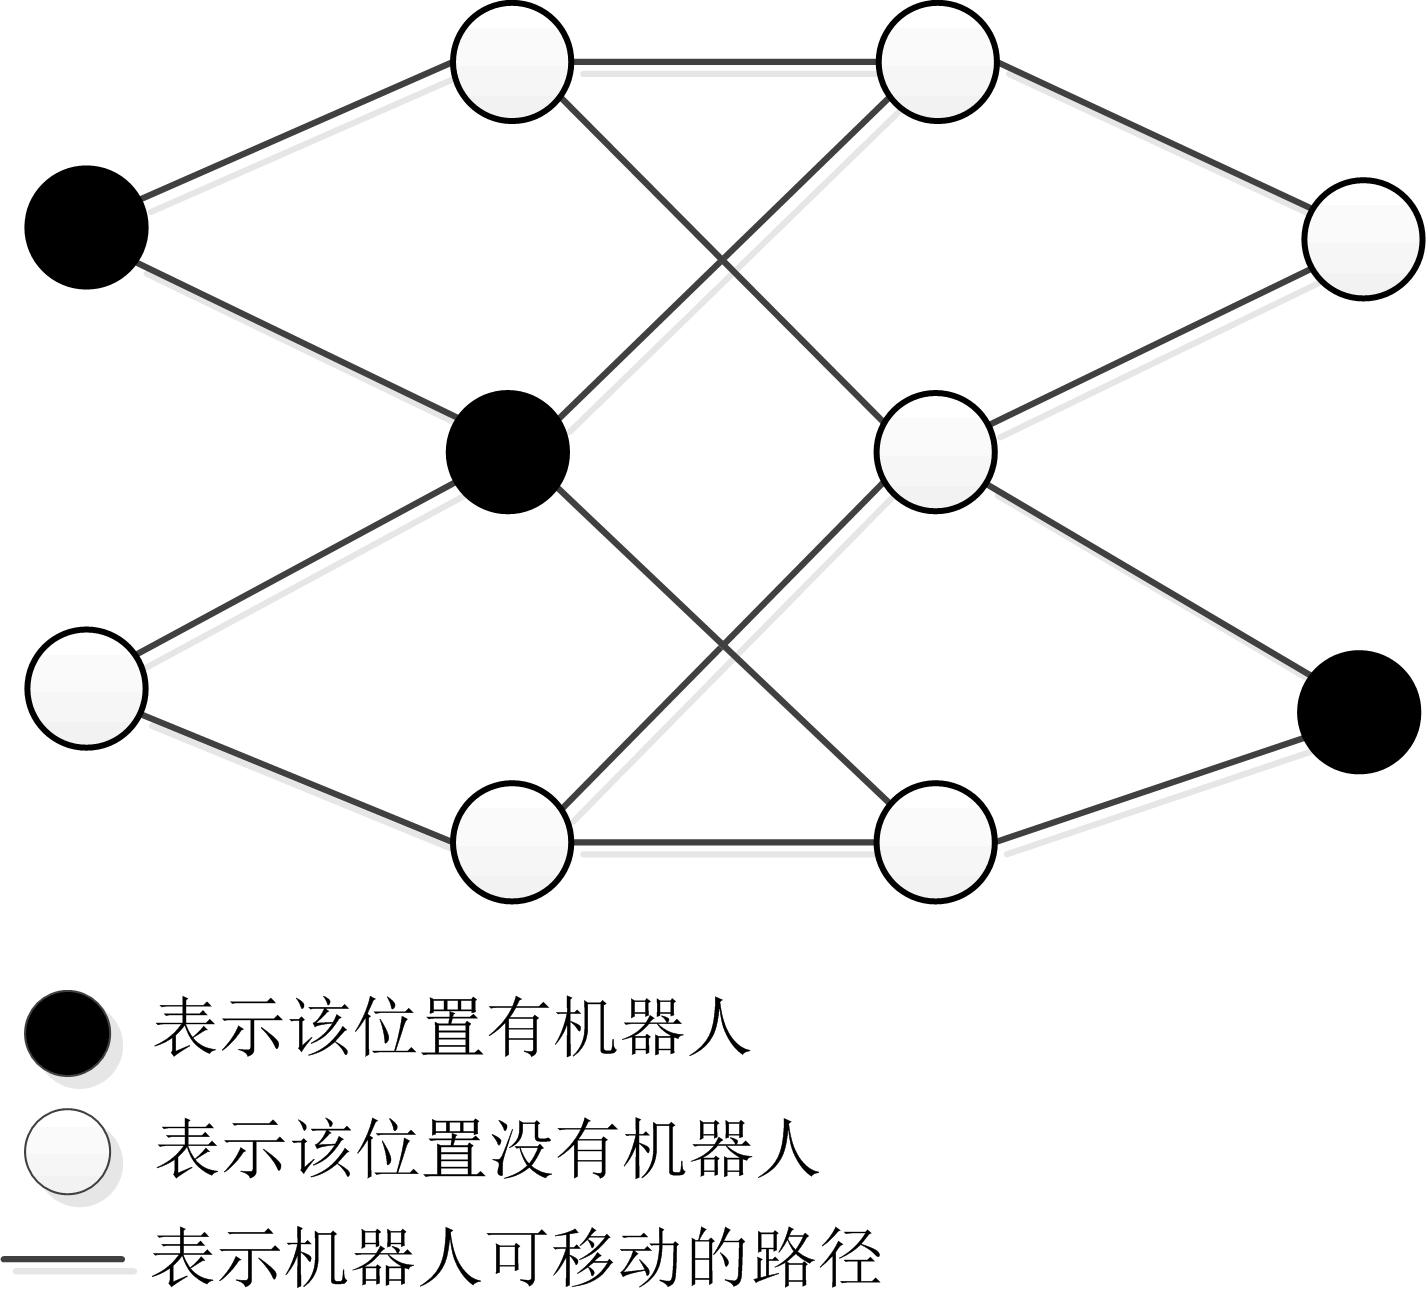
\includegraphics[width=3 in]{fig/normalspace.png}
	\caption{无向连通图表示探索空间}
	\label{fig:normalspace}
\end{figure}

如图\ref{fig:normalspace}是一个简单的离散空间模型,黑色结点表示该空间位置在此刻有一个机器人,白色结点说明该空间位置上没有机器人,空间中有三个机器人,分别位于三个黑色的空间位置结点上。离散空间的结构有很多,比如总线拓扑结构、星型拓扑结构、环形拓扑结构、树形拓扑结构等等。

\section{机器人移动}
在离散空间模型中,机器人可以沿着某条边从一个位置结点到达相邻的位置结点,如图\ref{fig:robotmove} 所示:

\begin{figure}[!hbt]
	\centering
	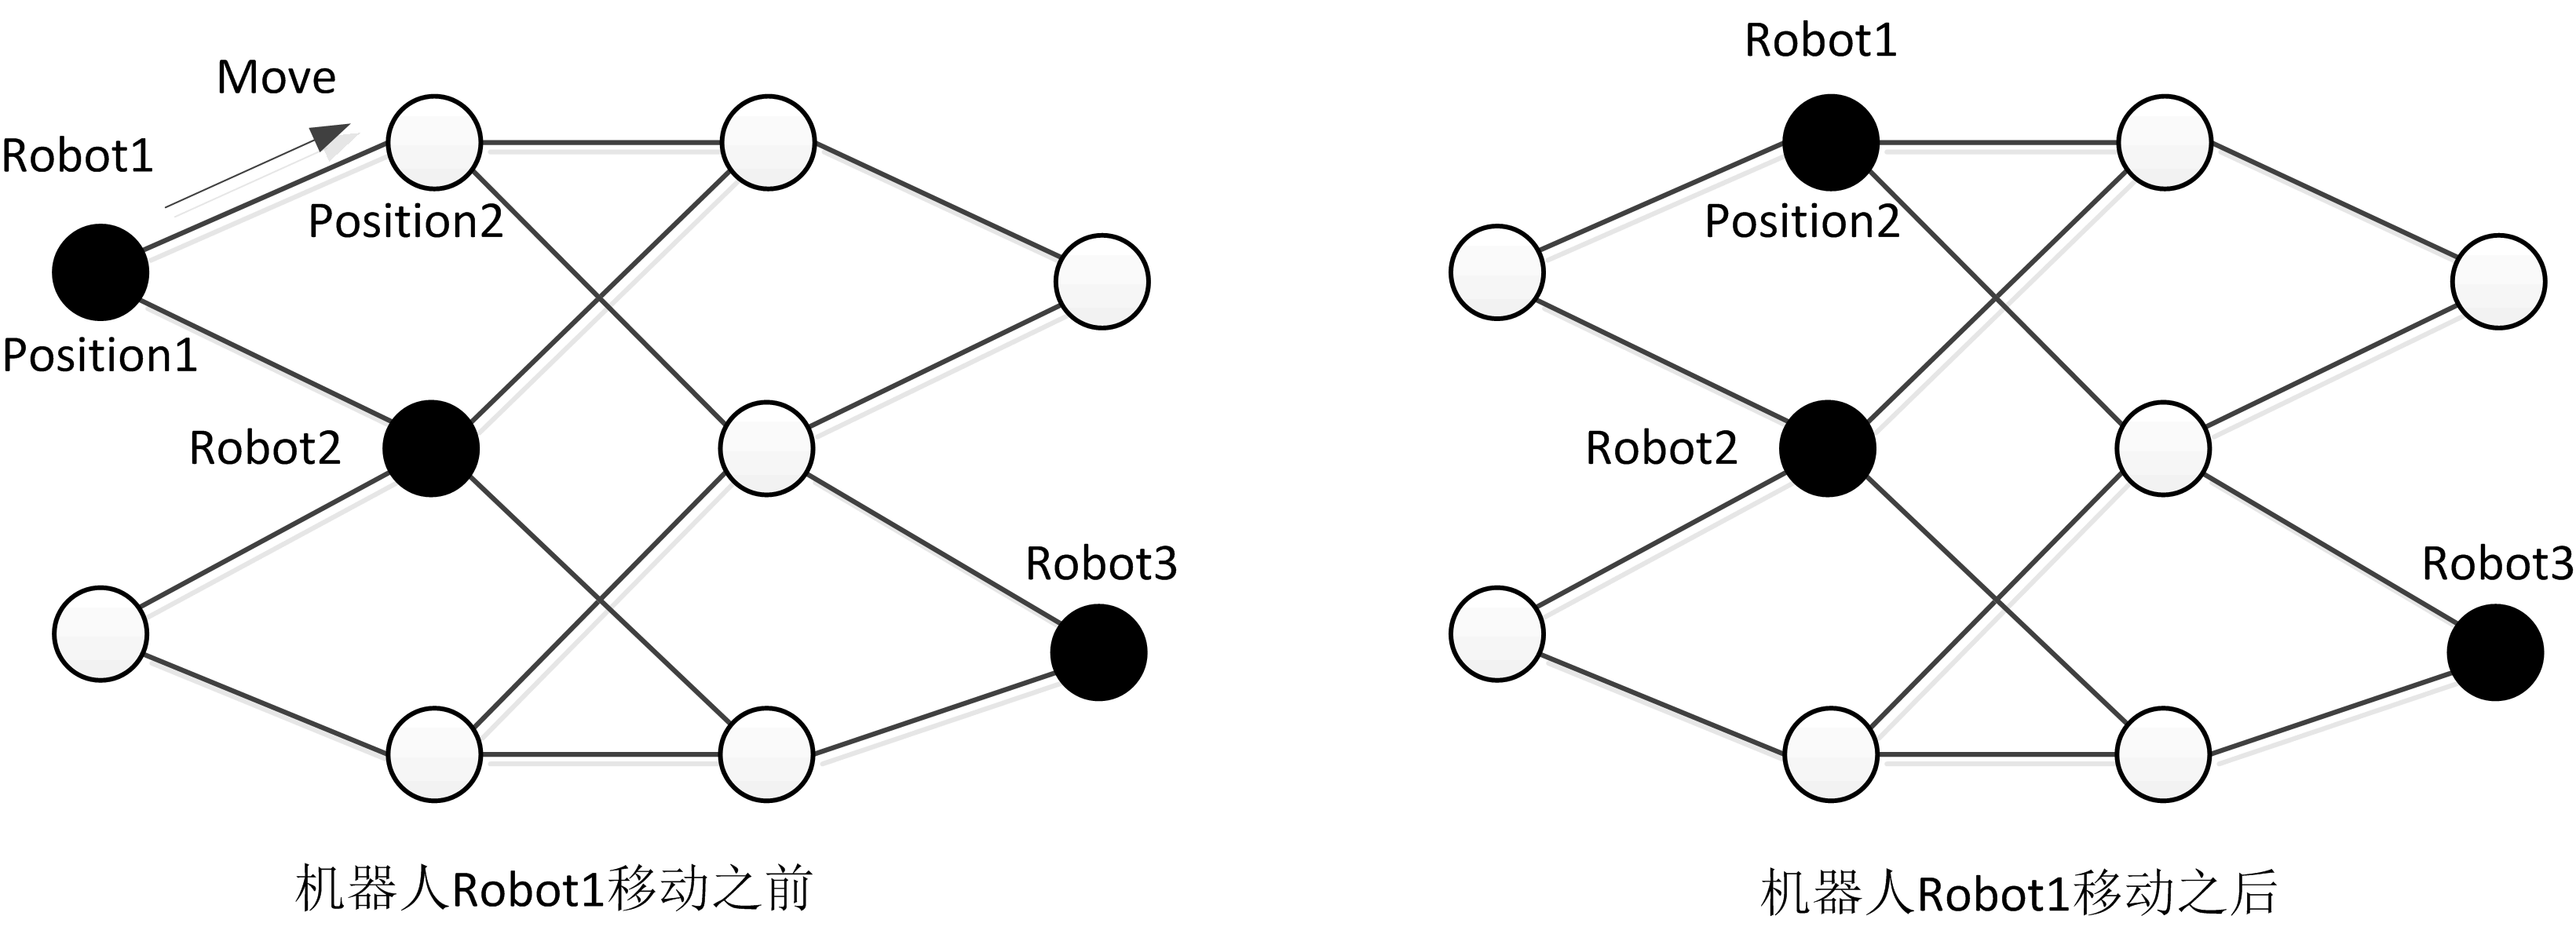
\includegraphics[width=5 in]{fig/robotmove.png}
	\caption{机器人在离散空间模型中的移动}
	\label{fig:robotmove}
\end{figure}

在位置结点Position1上的机器人Robot1沿着边移动,到达相邻的位置结点Position2上。相邻位置结点的定义是,两个位置结点通过一条边相连接,它们互为相邻位置结点,例如图中的位置结点Position1 和位置结点Position2 就是互为相邻位置结点。离散空间模型中的机器人移动两个基本特点:第一,有通往其他位置结点的边;第二,机器人每次移动之后,只能通过一条边,到达另外一个相邻位置结点之后,一个移动动作就完成,到达相邻位置结点之后,会重新开始一个移动动作。

自主移动机器人需要根据环境信息,匹配自身的移动算法做出移动决策,完成移动。如图\ref{fig:robotthreephase}机器人的移动动作可以分为三个阶段:观察(look)、计算(compute)和移动(move)。机器人在观察阶段,通过装备的视觉传感器,获取未知空间中其他机器人的位置快照。在计算阶段,通过匹配移动算法,获取机移动决策。在移动阶段,机器人的动力装置按照计算阶段获取移动决策完成移动。

\begin{figure}[!hbt]
	\centering
	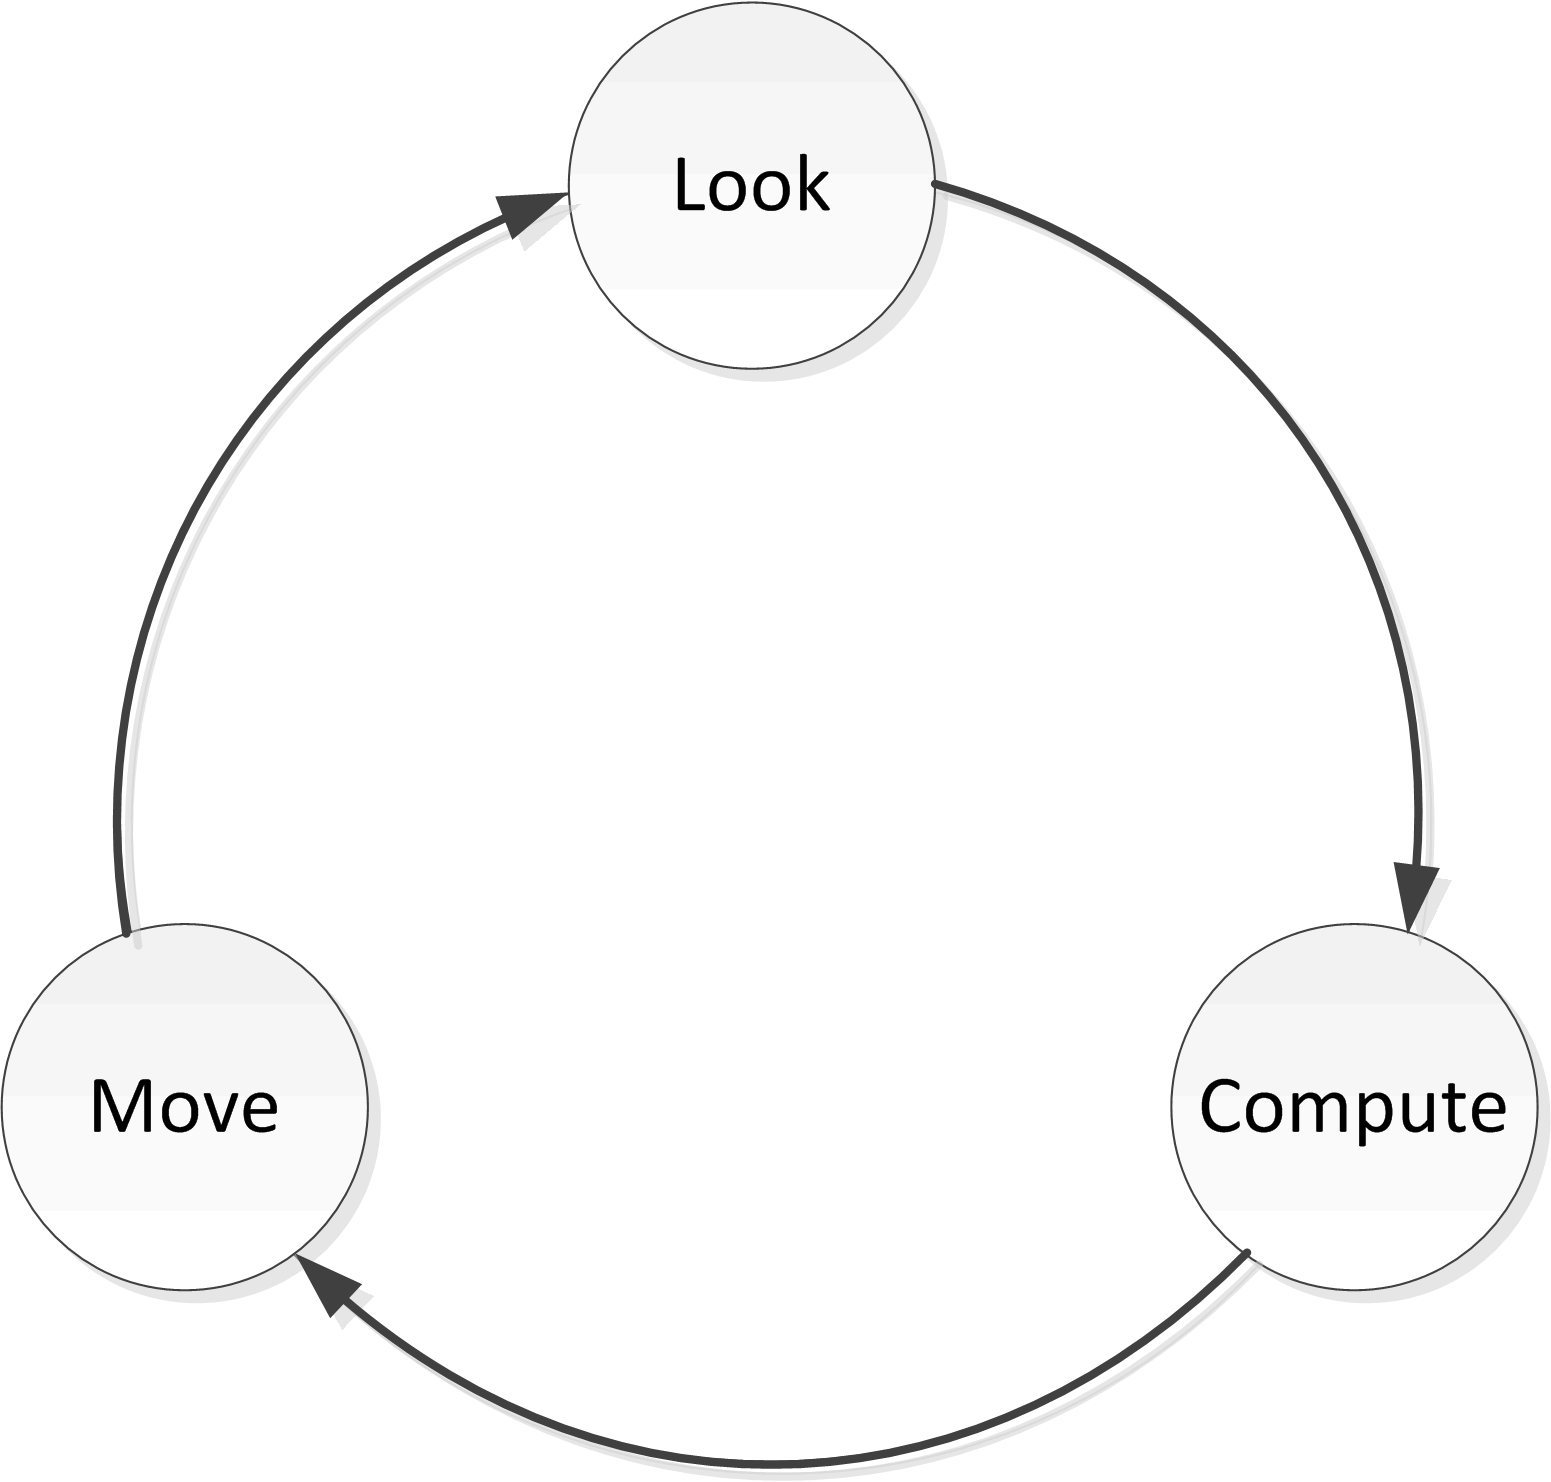
\includegraphics[width=2 in]{fig/robotthreephase.png}
	\caption{机器人移动三阶段}
	\label{fig:robotthreephase}
\end{figure}

机器人的观察、计算和移动是周期性重复进行的,当机器人完成移动之后,会进入观察阶段,获取周围的环境快照,快照匹配移动算法获取移动决策,在移动阶段完成移动,然后又进入观察阶段。

\section{调度策略}
在多自主移动机器人协作完成空间探索任务中,机器人调度是指机器人移动的三个阶段是否同步执行。假若有两个机器人A 和B,机器人A 在观察阶段时,机器人B也在观察阶段;机器人A在计算阶段时,机器人B 也在计算阶段;机器人A 在移动阶段时,机器人B 也在移动阶段,那么称机器人A和B是同步的,即机器人A和B的移动动作具备原子性。机器人的调度策略有三种:半同步调度策略\verb|(semi-synchronous model,SSYNC)|、完全同步调度策略\verb|(fully-synchronous model,FSYNC)|和完全异步调度策略\verb| (asynchronous model)|

为了方便描述调度策略,首先介绍以下几个概念。使用集合$Rob =\left\{k \in N^+ |r_1,r_2,r_3,...,r_k\right\}$ 表示未知空间中所有机器人,$k$是机器人个数,$r_k$表示机器人。使用集合$Pos =\left\{n \in N^+ |1,2,...,n\right\}$ 表示空间所有空间位置结点,$n$ 是空间位置结点个数,使用数字给空间中位置结点都进行了编号$1,2,...,n$。映射关系$c:\left\{Rob \rightarrow Pos\right\}$ 表示机器人所在的空间位置。机器人r 的空间位置定义为$c\left(r\right)$。 对于集合Rob 中的任意两个机器人$r_i,r_j\left(i \neq j \right)$, 在同一时刻满足$c\left(r_i\right) \neq c\left(r_j\right)$,即同一时刻,空间中任意一个位置结点上至多只有一个机器人。


\begin{figure}[!hbt]
	\centering
	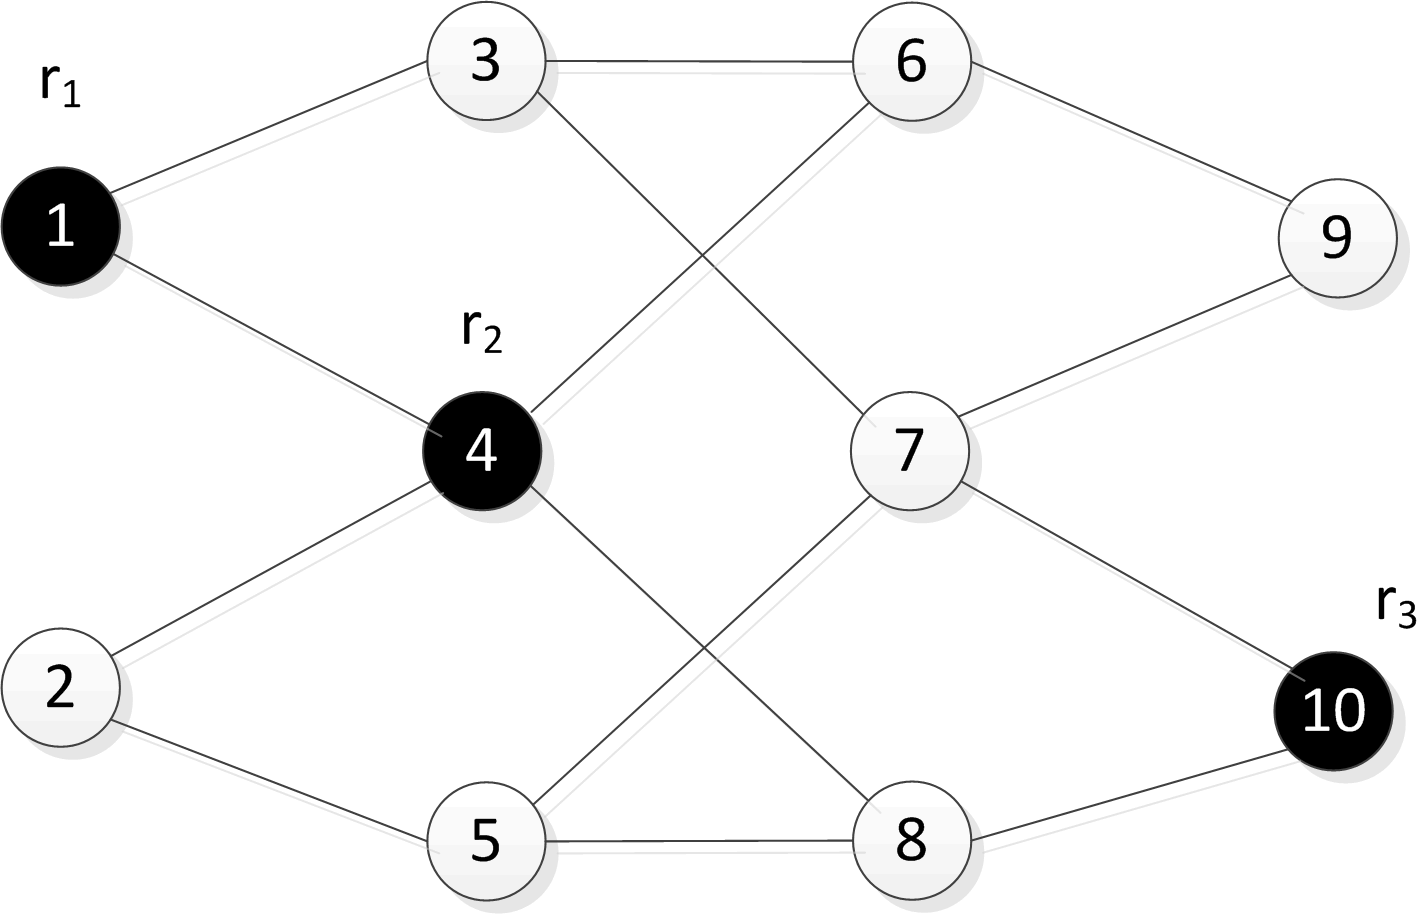
\includegraphics[width=2 in]{fig/robcollection.png}
	\caption{空间位置结点和机器人符号描述}
	\label{fig:robcollection}
\end{figure}

图\ref{fig:robcollection}中描述的离散空间中有三个机器人$r_1,r_2,r_3$,使用集合表示为$Rob =\left\{r_1,r_2,r_3\right\}$。 空间位置结点的集合为$Pos =\left\{n \in N^+ |1,2,3,4,5,6,7,8,9,10\right\}$。机器人$r_1$的位置表示为$c\left(r_1\right) = 1$,机器人$r_2$的位置表示为$c\left(r_2\right) = 4$,机器人$r_3$ 的位置表示为$c\right(r_3\right) = 10$。

\paragraph{半同步调度策略}
半同步调度策略中,只有被调度器选中的机器人,才会执行移动过程。为了方便描述,这里定义调度集合$Sched$,使用伪算法描述半同步调度策略:

\begin{lstlisting}
SSYNC-SCHEDULE(Rob)
  while
    choose Sched from Rob
    foreach r in Sched{
       synchronous {
          r.look
          r.compute
          r.move
       }
    }
\end{lstlisting}

伪算法的名称为\verb|SSYNC-SCHEDULE|表示半同步调度策略,空间中所有的机器人组成的集合$Sched$作为伪算法的参数参数。$choose \ Sched \ from \ Rob$表示从机器人集合$Rob$中选取一个子集$Sched$,并且子集$Sched$ 非空。\verb|foreach r in Sched|表示对于集合$Sched$中的每个机器人都同步执行观察、计算和移动过程。等移动完成之后,又进入下一个移动动作。在下一个移动动作开始之前,又重新选择调度子集$Sched$,\verb|while|表示重复上述机器人移动执行过程。这就是多机器人半同步调度策略的过程。

\paragraph{完全同步调度策略}
完全同步调度模型是半同步调度模型中一种很特殊的情况,每次移动动作之前选取调度子集$Sched$等于$Rob$,即每次调度的时候,集合$Rob$中的所有机器人都被选中。完全同步调度策略的伪算法描述如下:

\begin{lstlisting}
FSYNC-SCHEDULE(Rob)
   while
     foreach r in Rob{
        synchronous {
           r.look
           r.compute
           r.move
        }
     }
\end{lstlisting}

伪算法的名称为\verb|FSYNC-SCHEDULE|表示完全同步调度策略,除了$foreach \ r \ in \ Rob$这部分与半同步调度策略的伪算法不一样,其他部分都相同。由于每次选取的调度子集$Sched$等于$Rob$,所以这部分伪算法简化了调度过程,直接使用集合$Rob$作为调度集合。

\paragraph{完全异步调度策略}
完全异步调度策略中,所有的机器人观察、计算、移动都是异步,没有原子性。类似于计算机系统的多线程,每个机器人的移动都是并行且互相之间没有同步约束,当一个机器人处于观察阶段时,其他机器人可能处于计算阶段或者移动阶段。完全异步调度策略的伪算法如下:

\begin{lstlisting}
ASYNC-SCHEDULE(Rob)
    foreach r in Rob{
       asynchronous {
           while{
              r.look
              r.compute
              r.move
           }
       }
    }
\end{lstlisting}

伪算法的名称为\verb|ASYNC-SCHEDULE|,表示完全异步调度策略,关键字异步\verb|asynchronous|表示$Rob$中机器人是独立执行移动动作,执行观察、计算和移动的快慢,完全是自己执行速度所决定的。可能出现一种情况当某个机器人已经获取了空间环境快照,还未能执行计算或者移动时,其他机器人却完成了移动,改变了空间环境,这就会出现某些机器人使用过时环境信息,做出移动决策。\verb|while|表示在完全异步调度策略中,所有机器人都是不断循环的执行观察、计算和移动。

\section{环形空间探索算法}
未知空间结构有总线结构、星型结构、环形结构、树形结构等等。通常的研究是根据某种空间结构的特点,对空间进行建模与分析。本文使用环形空间为研究对象,详细介绍在环形空间中机器人的视觉快照和移动算法表示方法,以及移动算法匹配过程。最后,介绍一下环形空间最小移动算法。

\subsection{环形空间}
如图\ref{fig:ring1}是一个典型的环形空间模型,空间位置结点按照顺时针方向依次进行编号$1,2,3...,n$,图中有$n$个空间位置结点。

\begin{figure}[!hbt]
	\centering
	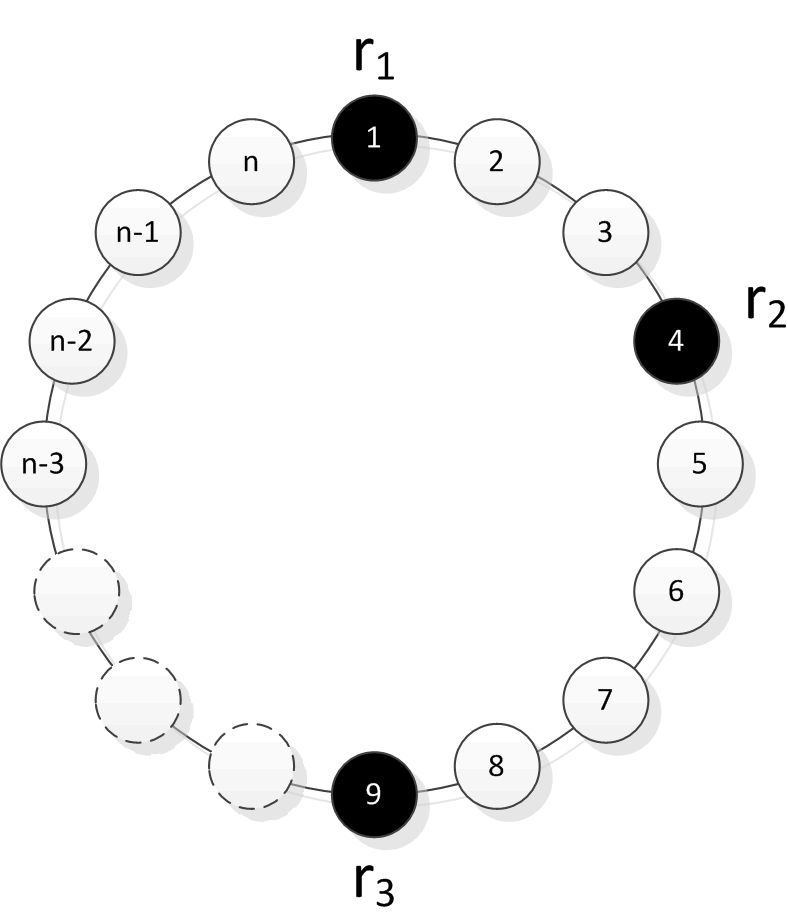
\includegraphics[width=2 in]{fig/ring1.png}
	\caption{环形空间}
	\label{fig:ring1}
\end{figure}

环形空间中位置结点的集合表示为$Pos =\left\{1,2,...,n\right\}$,环形空间有自身的一些特点:1、每个空间位置结点都有左右两个相邻的位置结点,例如位置结点$1$的左边(逆时针)是位置结点$n$,右边(顺时针)是位置结点$2$。2、每个空间位置与左右相邻的位置结点,都有各自有条边(路径)连通。3、机器人每次移动,只能顺时针或者逆时针进行移动。例如图中机器人$r_1$可以顺时针移动到位置结点$2$, 也可以逆时针移动到位置结点$n$。环形空间中的位置结点上,也必须是在同一时刻至多只能有一个机器人。

\subsection{环境快照}
机器人可以通过视觉传感器获取环境快照,在环形空间中,可以沿着顺时针或者逆时针方向,获取环境快照。对于机器人而言,只能判断某个空间位置结点上是否有机器人。

\begin{figure}[!hbt]
	\centering
	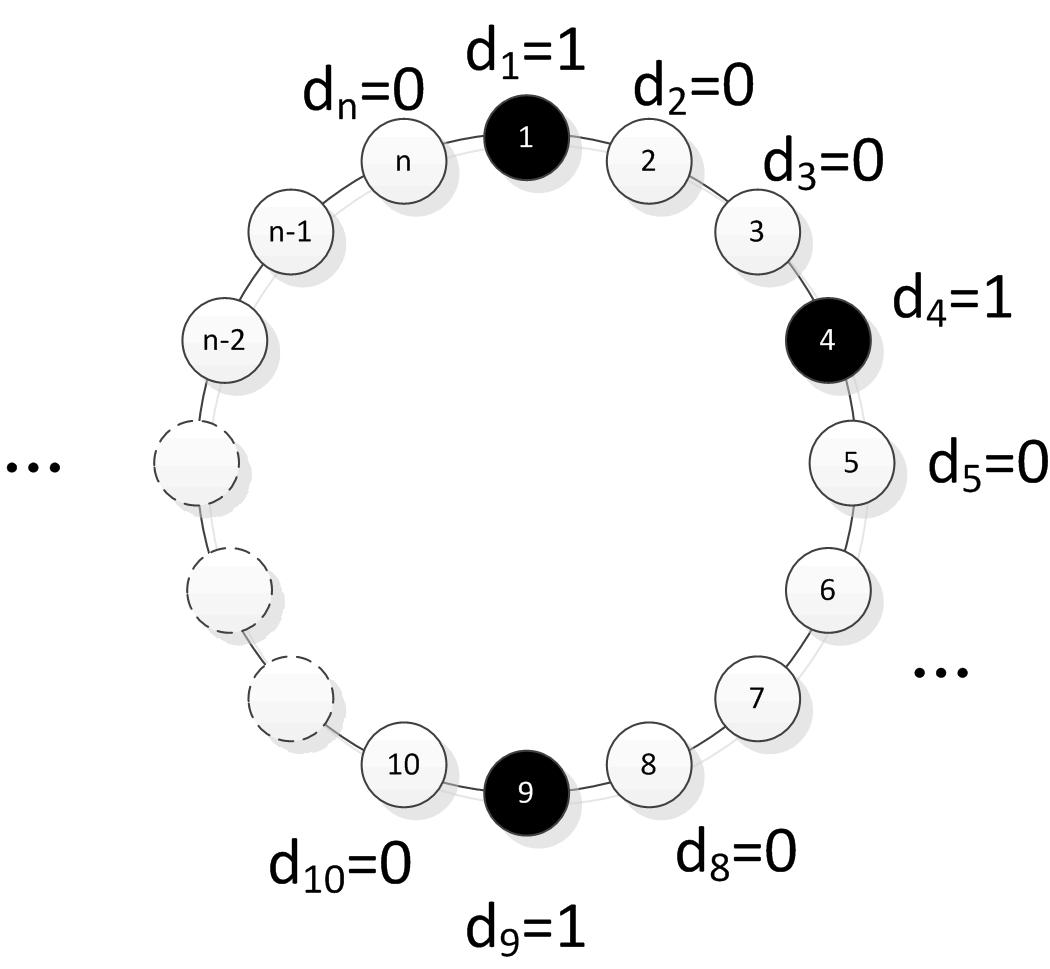
\includegraphics[width=3.5 in]{fig/snapshot1.png}
	\caption{结点机器人的描述}
	\label{fig:snapshot1}
\end{figure}

如图\ref{fig:snapshot1}使用符号$d_j$表示空间位置结点$j$上是否有机器人,其中$j \in Pos $。当空间位置结点$j$上,有机器人时,那么$d_j = 1$,表示该空间位置结点上有$1$个机器人。当空间位置结点上没有机器人时,那么$d_j = 0$,表示该空间位置结点上有$0$个机器人。

假设在空间位置$j$上有一个机器人$r$,即$ d_j = 1 \land c\left(r\right) = j$。使用符号$\delta_{c\left(r\right)}^F$ 表示机器人$r$的环境快照,其中\verb|F|表示机器人获取环境快照的方向,$F \in \left\{+,-\right\}$,\verb|+|表示顺时针,\verb|-| 表示逆时针。

在有\verb|n|个位置结点的环形空间上,空间位置结点\verb|j|上机器人r的顺时针和逆时针环境快照如下:

\verb|顺时针环境快照:| $\delta_{c\left(r\right)}^+ = \left\langle d_j,d_{j+1},...,d_{j+n-1}  \right\rangle.$

\verb|逆时针环境快照:| $\delta_{c\left(r\right)}^- = \left\langle d_j,d_{j-1},...,d_{j-n+1}  \right\rangle.$

具体看一个实例,在图\ref{fig:snapshot1}中空间位置结点\verb|1|上的机器人顺时针和逆时针环境快照如下:

\verb|顺时针环境快照:| $\delta_1^+ = \left\langle 1,0,0,1,0,0,0,0,1,0,... \right\rangle.$

\verb|逆时针环境快照:| $\delta_1^- = \left\langle 1,0,...,0,1,0,0,0,0,1,0,0 \right\rangle.$

使用上述环境快照表达方式,比较直接、简洁。但是当环形空间中位置结点数较多或者未知时,这种表达式就十分长,不容易书写或者存储。\verb|F-R|表达式\cite{r5}描述环境快照就可以很好的避免这些问题,\verb|F-R| 表达方式中使用$F_m$ 表示连续m个没有机器人空间位置结点数,$R_n$表示连续\verb|n|个有机器人空间位置结点数。

\begin{figure}[!hbt]
	\centering
	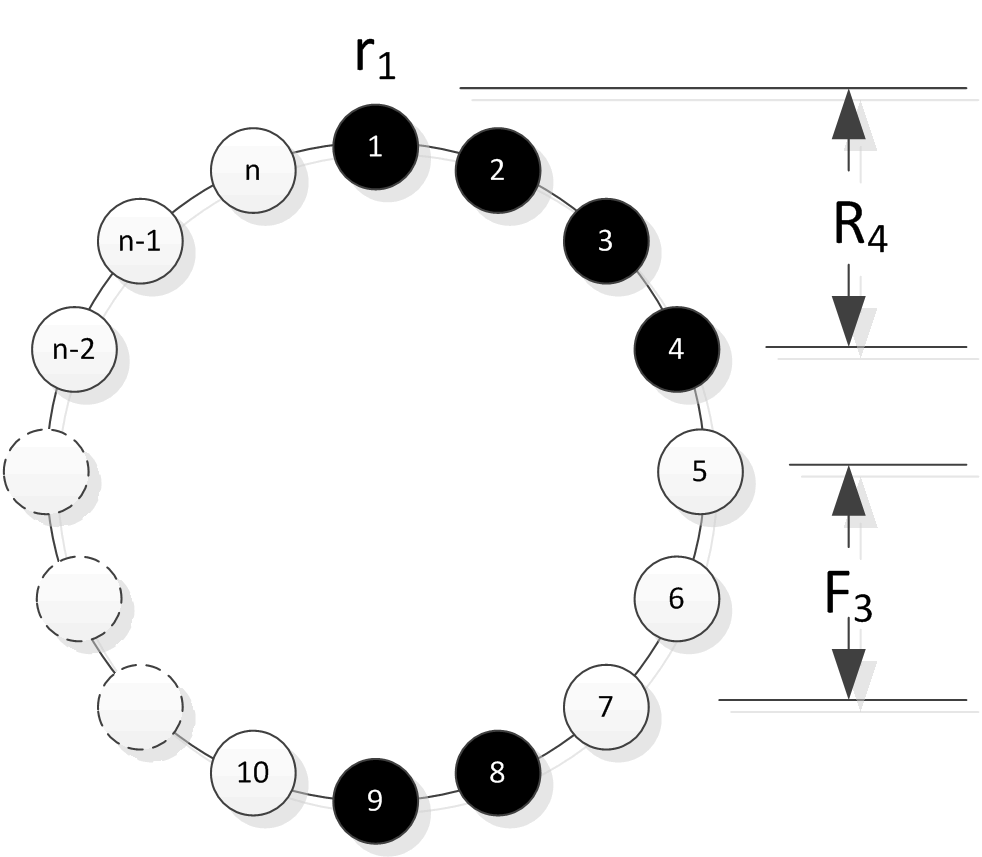
\includegraphics[width=3.5 in]{fig/frsnapshot.png}
	\caption{环形空间F-R快照表达式}
	\label{fig:frsnapshot}
\end{figure}

图\ref{fig:frsnapshot}中有\verb|n|个机器人,机器人$r_1$顺时针方向,有连续4个空间位置上有机器人,可以使用$R_4$ 表示。紧跟顺时针方向又有连续的三个无机器人的空间位置结使用$F_3$表示。那么在空间位置结点$1$的上的机器人$r_1$的顺时针\verb|F-R| 快照表达式为$\delta_{c\left(r_1\right)}^+ = \left\langle R_4,F_3,R_2,F_{n-9}\right\rangle$。 可以看出在\verb|F-R| 快照表达式中,使用具体整数或者未知参数表示连续的空间位置,这样的描述不仅缩短了表达式的长度,而且描述能力更强。当在未知环形空间位置结点数量,\verb|F-R|快照表达式也可以很方便的进行描述。

\subsection{对称性}
环形空间中,机器人的位置关系可能会出现对称性的情况。若是出现对称,可能导致某个机器人的顺时针和逆时针环境快照完全相同,或者两个对称的机器人环境快照相同。

\begin{figure}[!hbt]
	\centering
	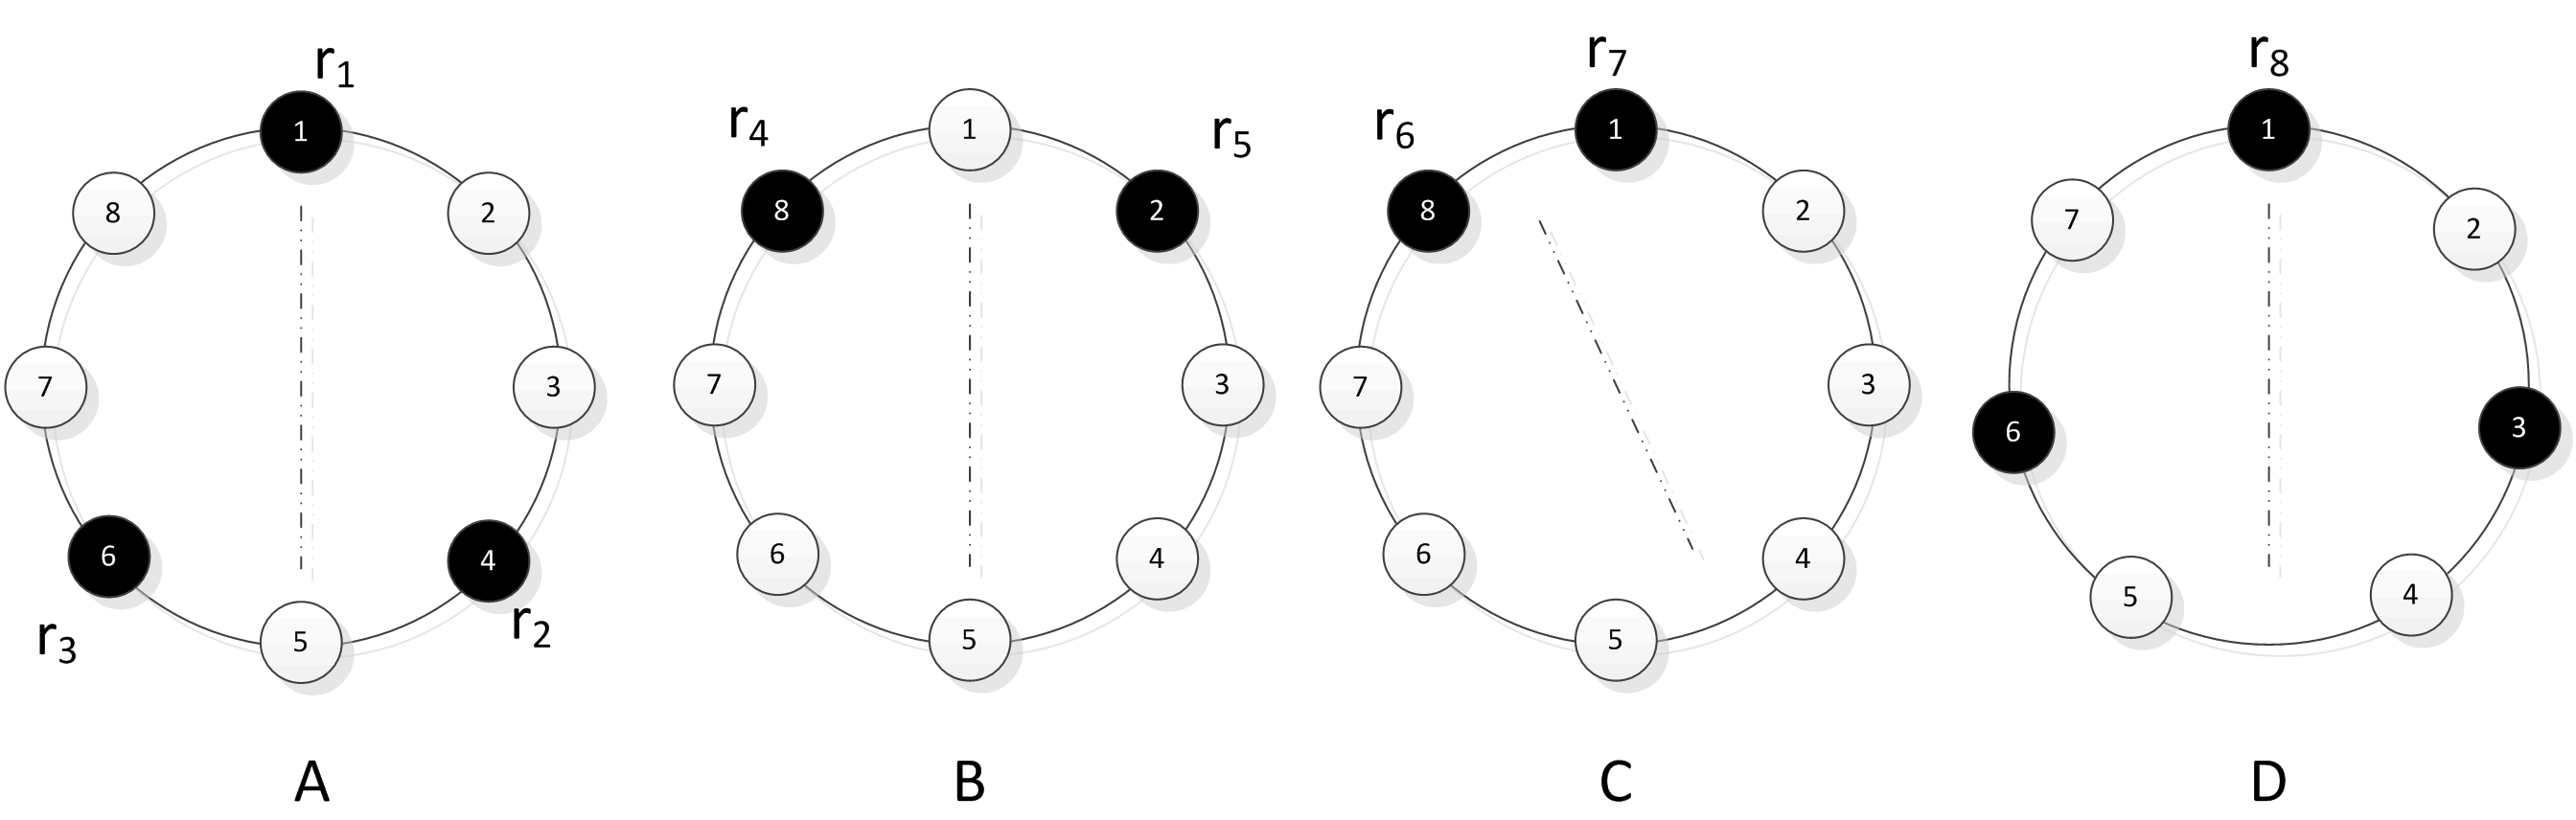
\includegraphics[width=3.5 in]{fig/symmetric.png}
	\caption{环形空间对称}
	\label{fig:symmetric}
\end{figure}

如图\ref{fig:frsnapshot},有四组对称环形空间模型,A中机器人$r_1$的顺时针和逆时针F-R快照表达式为:

 $\delta_{c\left(r_1\right)}^+ = \left\langle R_1,F_2,R_1,F_1,R_1,F_2 \right\rangle.$

 $\delta_{c\left(r_1\right)}^- = \left\langle R_1,F_2,R_1,F_1,R_1,F_2 \right\rangle.$

 可以看出$\delta_{c\left(r_1\right)}^+$和$\delta_{c\left(r_1\right)}^-$完全相同。B中机器人$r_4$和$r_5$,B中机器人$r_6$和$r_7$是对称的。A中位置结点个数是偶数,D中位置结点个数是奇数,表明环形空间位置结点数,无论是奇数还是偶数,都可能会出现对称的情况。

\subsection{移动算法}
在环形空间中,机器人有三种可能的移动策略:不移动,顺时针移动、逆时针移动。而对于无方向识别能力的机器人而言,其移动策略只能依据当前环境快照做出前进或者后退的移动策略。而环形空间具有对称性,所以机器人的移动策略有四种:$\left(Idle\right)$、 前进$\left(Front\right)$、 后退$\left(Back\right)$、 未确定$\left(Doubt\right)$。移动策略集合$MOVE = \left\{Idle,Front,Back,Doubt\right\}$。其中\verb|Doubt|表示机器人可以前进或者后退。

移动算法是一组移动规则,移动规则使用符号\verb|L|表示,其结构如下:

 $ L :\delta_{c\left(r\right)}^F  \rightarrow  r.MOVE $

机器人\verb|r|的环境快照与\verb|L|的$\delta_{c\left(r\right)}^F$匹配时,机器人\verb|r|就执行移动规则\verb|L|中的移动决策$MOVE$。

下面通过最小移动算法\cite{r5}的介绍,可以更详细的了解移动算法。最小移动算法是环形空间中使用最少的机器人完成未知空间永恒探索\cite{r5}。具体最小移动算法的条件是空间位置结点数$n \geq 10$,机器人数$k = 3$,且\verb|n|与\verb|k|互质。最小移动算法分为两个阶段:稳定阶段$\left(Legitimate\quad phase\right)$ 和收敛阶段$\left(Convergence\quad phase\right)$。

\begin{table}[hbt]
    \centering
    \caption{最小移动算法稳定阶段}
    \begin{tabular}{|p{2cm}|p{8cm}|p{2cm}|p{2cm}|}
        \hline
        $RL1$&$\delta_{c\left(r\right)}^F = \left\langle R_2,F_2,R_1,F_{n-5} \right\rangle.$&$\rightarrow$&$r.Back$\\
        \hline
        $RL2$&$\delta_{c\left(r\right)}^F = \left\langle R_1,F_1,R_1,F_{n-6},R_1,F_2 \right\rangle.$&$\rightarrow$&$r.Front$\\
        \hline
        $RL3$&$\delta_{c\left(r\right)}^F = \left\langle R_1,F_3,R_2,F_{n-6}\right\rangle.$&$\rightarrow$&$r.Front$\\
        \hline
    \end{tabular}
    \label{table:minalgotithm}
\end{table}

\vspace{0.5cm}

\begin{figure}[!hbt]
	\centering
	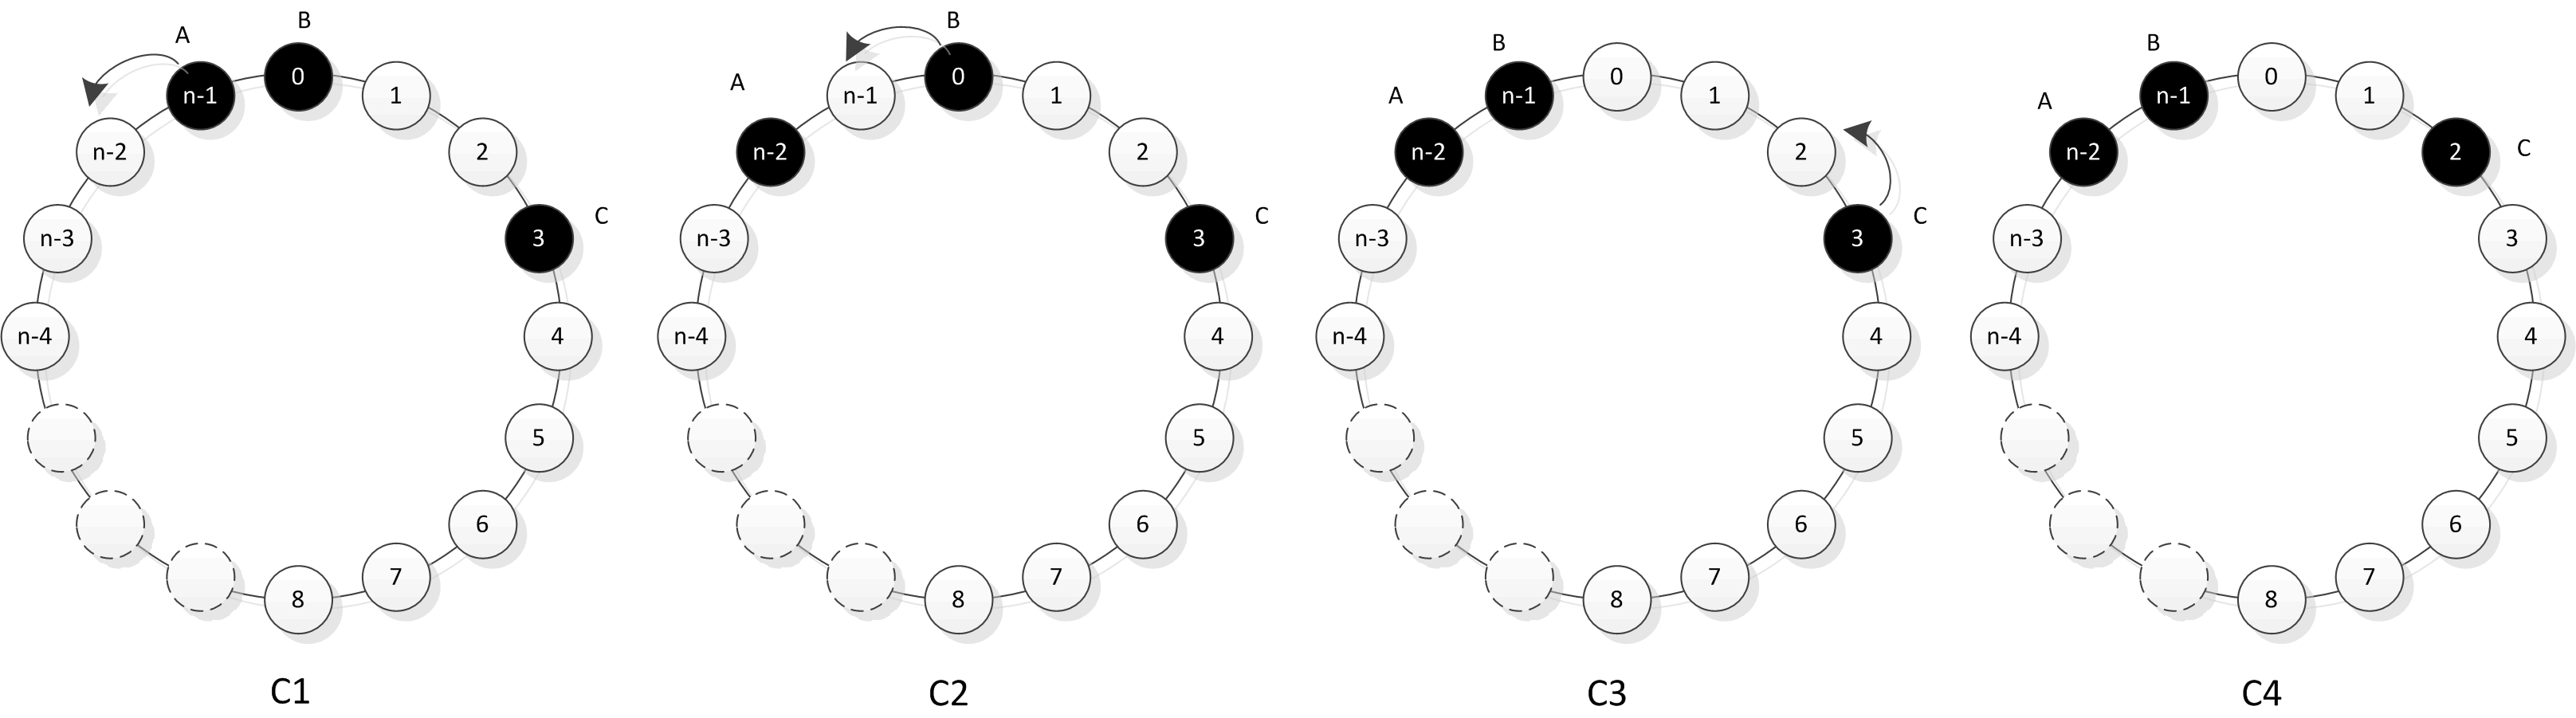
\includegraphics[width=6.5 in]{fig/perpetualexploration.png}
	\caption{最小移动算法的稳定阶段}
	\label{fig:perpetualexploration}
\end{figure}

在图\ref{fig:perpetualexploration}中,所有机器人是依据最小移动算法执行移动。C1 中机器人A 的顺时针环境快照$\delta_{c\left( A\right)}^+$ 匹配移动算法$RL1$ 做出后退的移动决策,机器人A 从位置结点$n-1$移动到$n-2$, 其他机器人$B$ 和$C$此时没有匹配任何移动算法,保持静止。C2 中机器人B 的逆时针环境快照${delta_{c\left( B\right)}^-}$ 匹配移动算法$RL2$,做出前进的移动决策,机器人A从位置结点$0$ 移动到$n-1$。 同样机器人C 的逆时针环境快照,匹配移动$RL3$ 做出前进的移动决策,从位置结点$3$ 移动到$2$。此时,\verb|C4|相对于\verb|C1|是所有的机器人向顺时针方向移动了一个位置。\verb|C4|和\verb|C1|所有机器人的环境快照完全相同。意味着所有机器人会按照上述C1到C4过程重复执行移动过程。

像这样所有机器人在某一个状态开始,循环执行一组移动规则,而且在移动规则下,所有机器人都向某一个固定的方向移动,称为稳定阶段。相对于稳定阶段的是收敛阶段:

\begin{table}[hbt]
    \centering
    \caption{最小移动算法收敛阶段}
    \begin{tabular}{|p{2cm}|p{8cm}|p{1cm}|p{2cm}|}
        \hline
        $RC1$&$4 \leq x \leq z  \land \delta_{c\left(r\right)}^F = \left\langle R_1,F_x,R_2,F_z\right\rangle.$&$\rightarrow$&$r.Front$\\
        \hline
        $RC2$&$x \neq y,x>0 \land \delta_{c\left(r\right)}^F = \left\langle R_1,F_x,R_1,F_y,R_1,F_x\right\rangle.$&$\rightarrow$&$r.Doubt$\\
        \hline
        $RC3$&$0<x<z<y \land \left( x,y \right) \neq  \left( 1,2 \right)\land \delta_{c \left(r\right)}^F = \left\langle R_1,F_3,R_2,F_{n-6}\right\rangle.$&$\rightarrow$&$r.Front$\\
        \hline
        $RC4$&$\delta_{c\left(r\right)}^F = \left\langle R_3,F_{n-3}\right\rangle.$&$\rightarrow$&$r.Back$\\
        \hline
        $RC5$&$\delta_{c\left(r\right)}^F = \left\langle R_1,F_1,R_2,F_{n-4}\right\rangle.$&$\rightarrow$&$r.Back$\\
        \hline
    \end{tabular}
    \label{table:minalgotithmconvergence}
\end{table}

在表\ref{fig:minalgotithmconvergence}中是最小算法的收敛阶段。在未知空间中,机器人的初始位置可以是任意的,机器人通过收敛阶段可以到达稳定阶段。

\begin{figure}[!hbt]
	\centering
	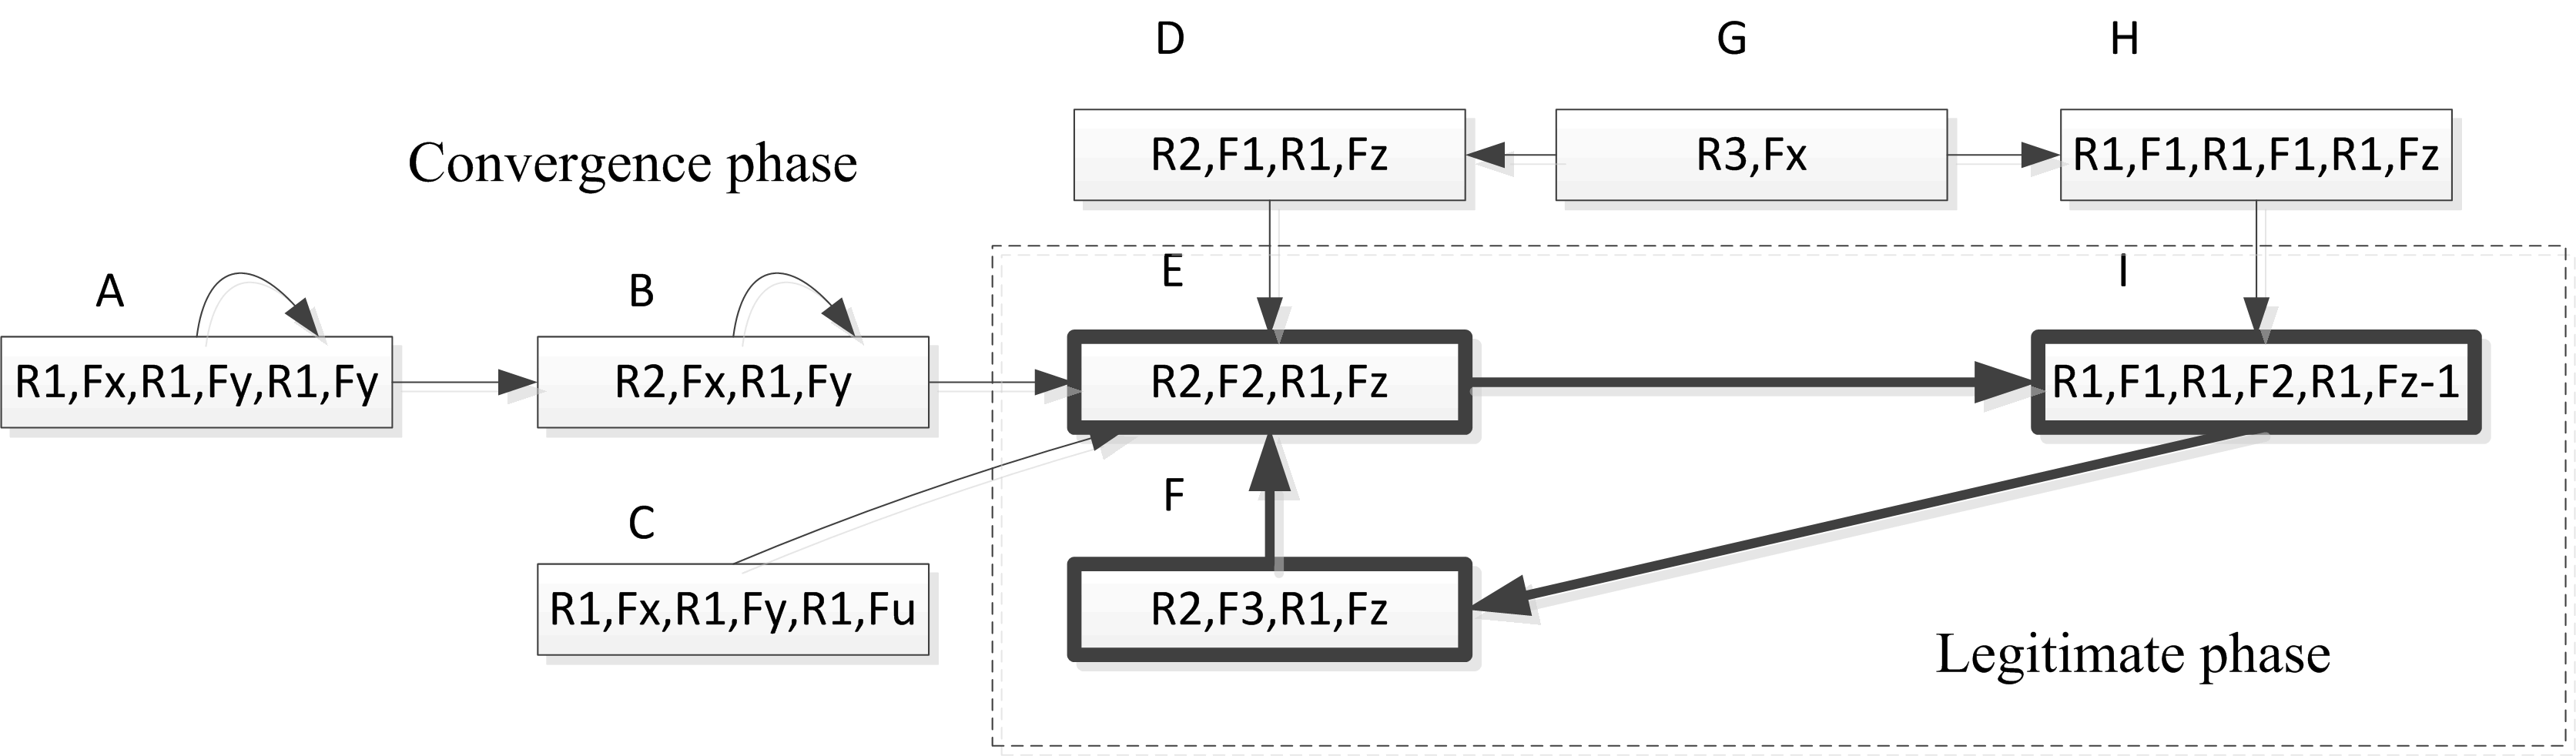
\includegraphics[width=6 in]{fig/cp_lp.png}
	\caption{稳定阶段和收敛阶段}
	\label{fig:cp_lp}
\end{figure}

通过图\ref{fig:cp_lp}来解释最小移动算法的收敛阶段和稳定阶段。图中每个长方形块表示整个环形空间可能出现的环境状态。收敛阶段使用集合\verb|LC|表示,集合$LC$包含$\left\{A,B,C,D,G,H\right\}$环境状态。稳定阶段环境使用集合\verb|RL|表示,集合$RL$包含$\left\{E,F,I\right\}$环境状态。图中包含了所有最小移动算法中,机器人所有可能初始的位置。

下面详细介绍一下\verb|E|到\verb|I|的状态变化过程,状态变化过程也基本相同,可以参照理解。

\begin{figure}[!hbt]
	\centering
	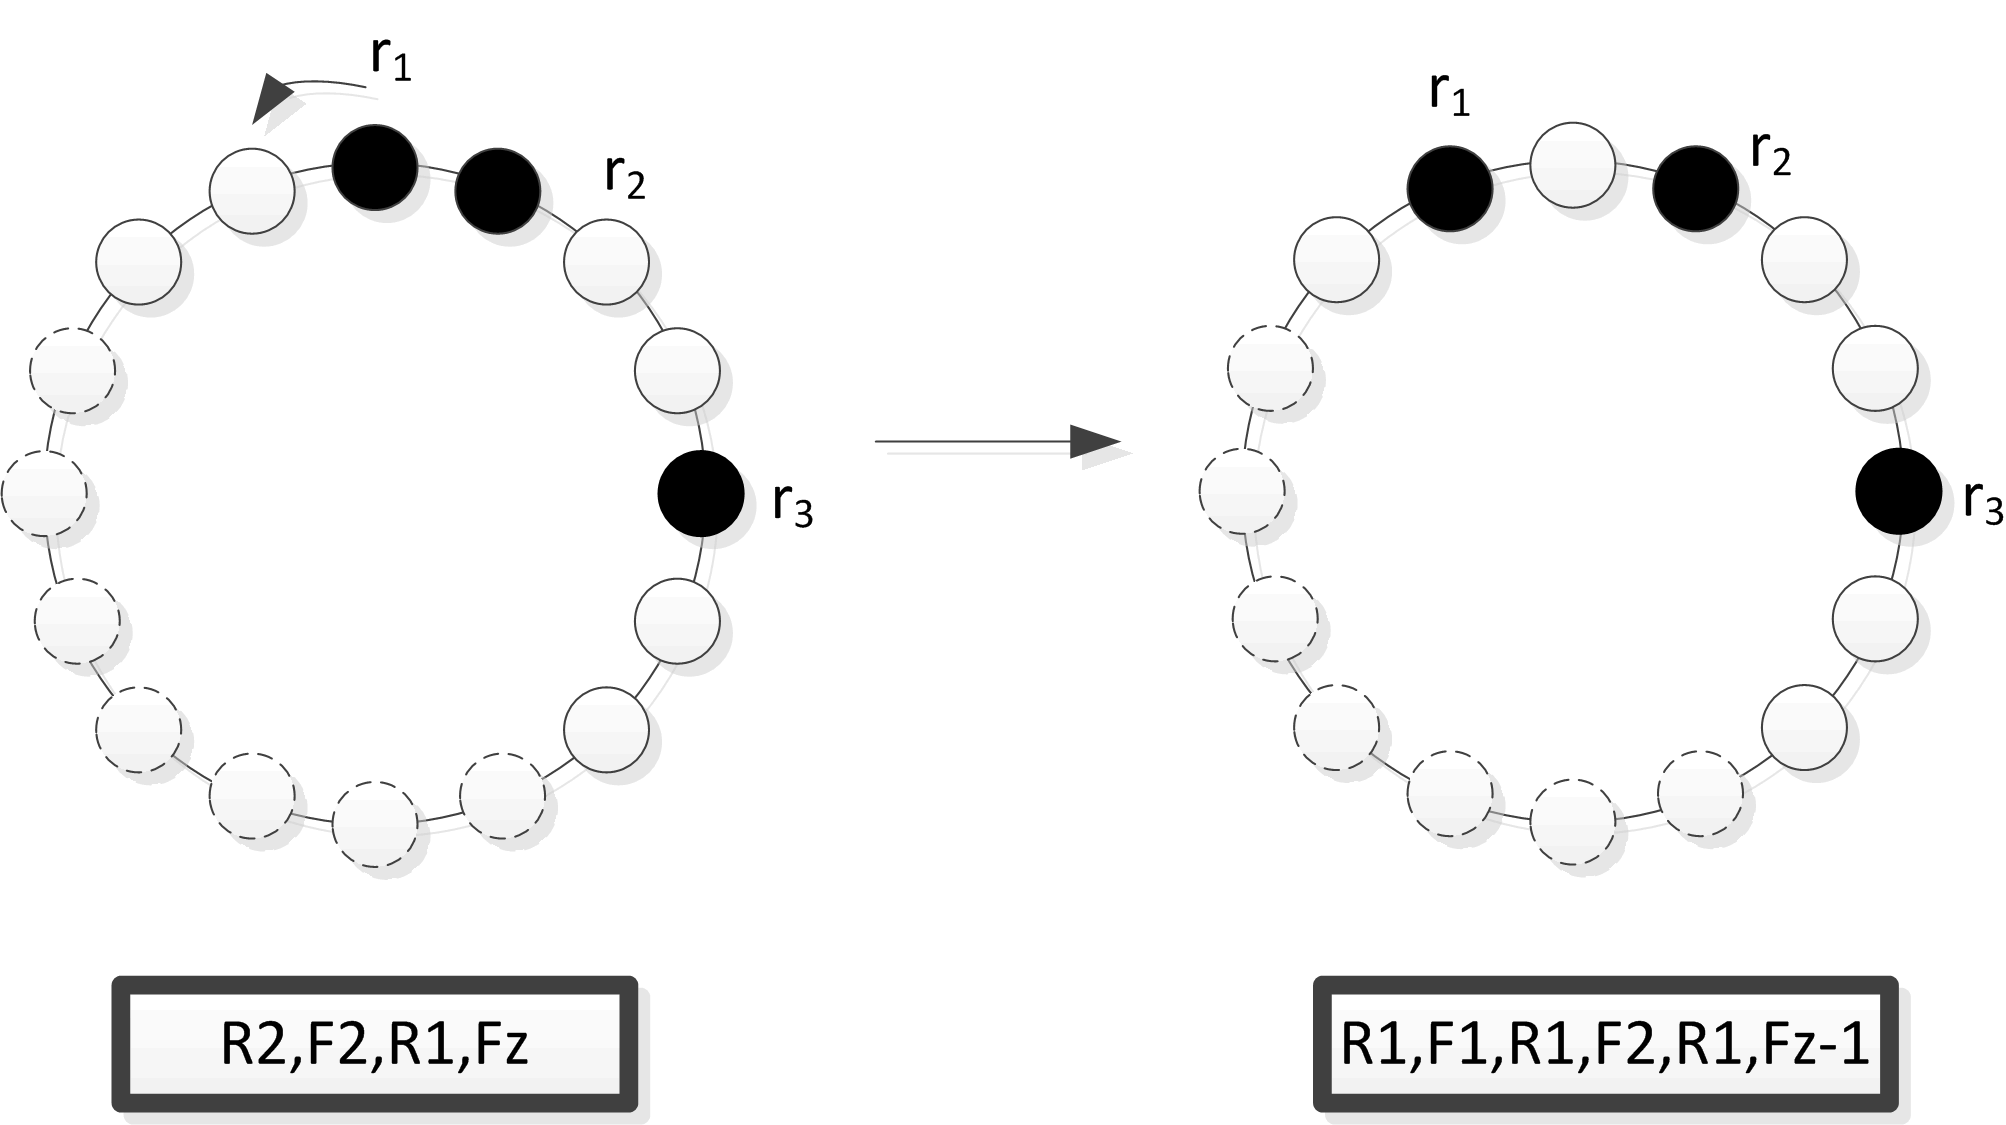
\includegraphics[width=5 in]{fig/stateexchange.png}
	\caption{环境快照状态变化}
	\label{fig:stateexchange}
\end{figure}

环境状态$R2,F2,R1,Fz$变化$R1,F1,R1,F2,R1,Fz-1$的过程中,是由于机器人$r_1$匹配移动规则$RL_1$之后,做出向后移动决策。由此可知图\ref{fig:cp_lp}中是由于机器人的移动,导致环境状态的变化。

由图\ref{fig:cp_lp}可知,最小移动机器人算法中所有的非稳定状态,都可以通过收敛阶段到达稳定状态。进入稳定状态之后,就不会回到收敛状态。稳定状态是一个闭环图,进入稳定状态之后,所有机器人都循环执行稳定阶段的移动算法。

\section{永恒探索}
永恒探索是空间中所有机器人满足对空间中所有位置结点进行重复访问的性质。永恒探索只是移动算法满足非冲撞性(No collision),非互换性(No switch),非终止性(Live)。

\subsection{非冲撞性}
冲撞是指在环形空间中,某个空间位置结点上,同一时刻有2个或者更多的机器人。

\begin{figure}[!hbt]
	\centering
	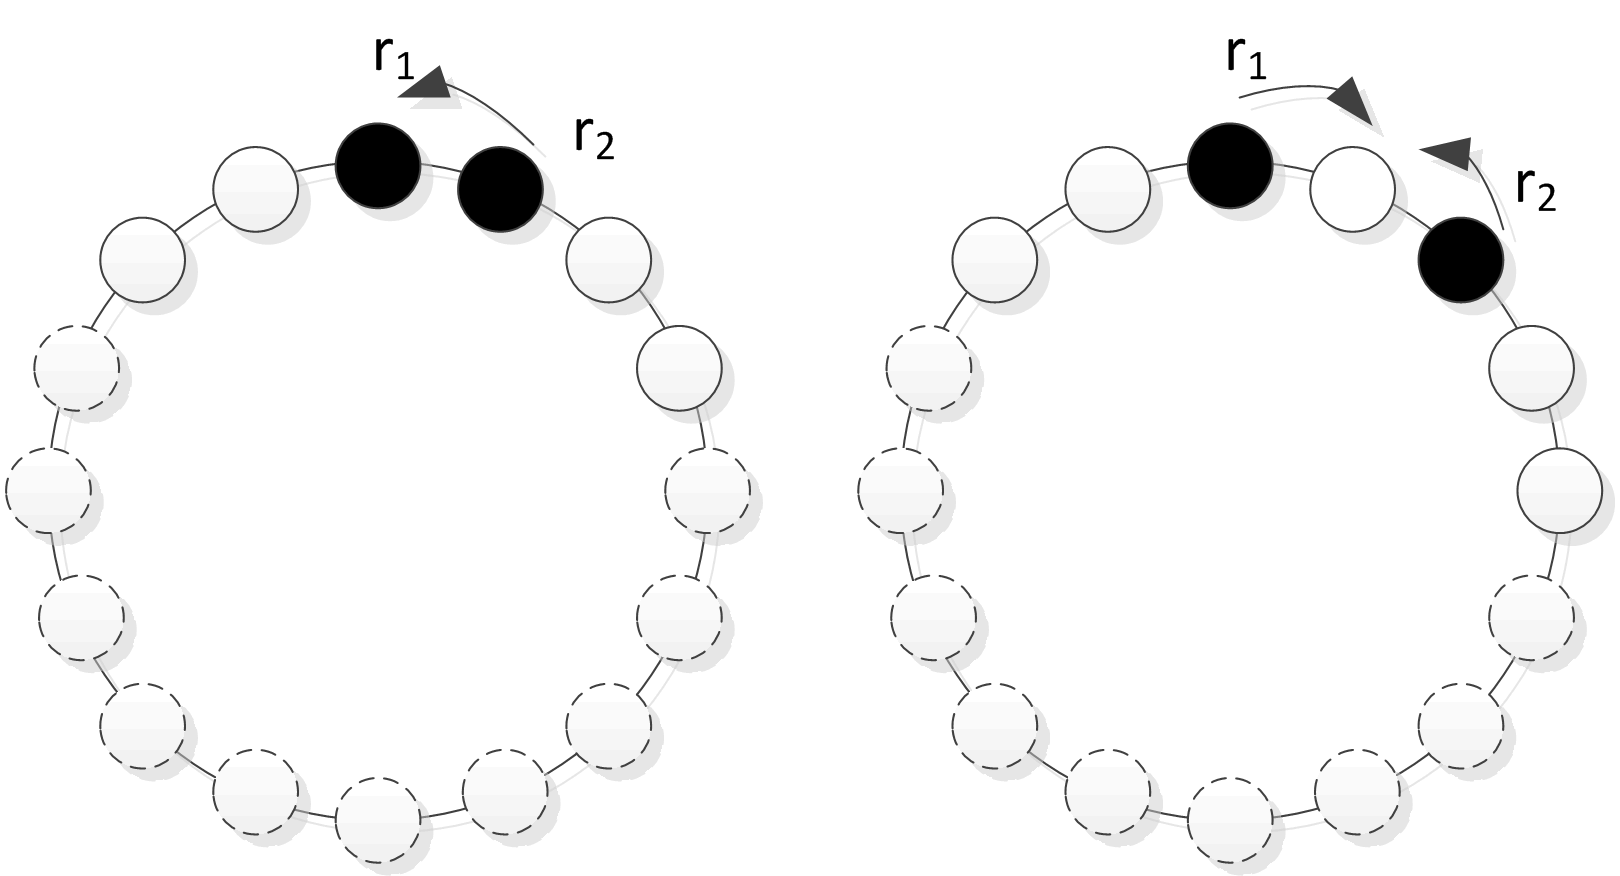
\includegraphics[width=5 in]{fig/collision.png}
	\caption{冲撞}
	\label{fig:collision}
\end{figure}

如图\ref{fig:collision}所示,当机器人$r_2$移动到机器人$r_1$所在空间位置结点或者机器人$r_1$和$r_2$同时移动到同一个空间位置结点时,就会发生碰撞,所谓非冲撞性,则是指所有机器人移动过程中,永远不会发生冲撞。

\subsection{非互换性}
互换是指相邻的两个机器人,下一个状态时,它们所在的空间位置发生的互换。

\begin{figure}[!hbt]
	\centering
	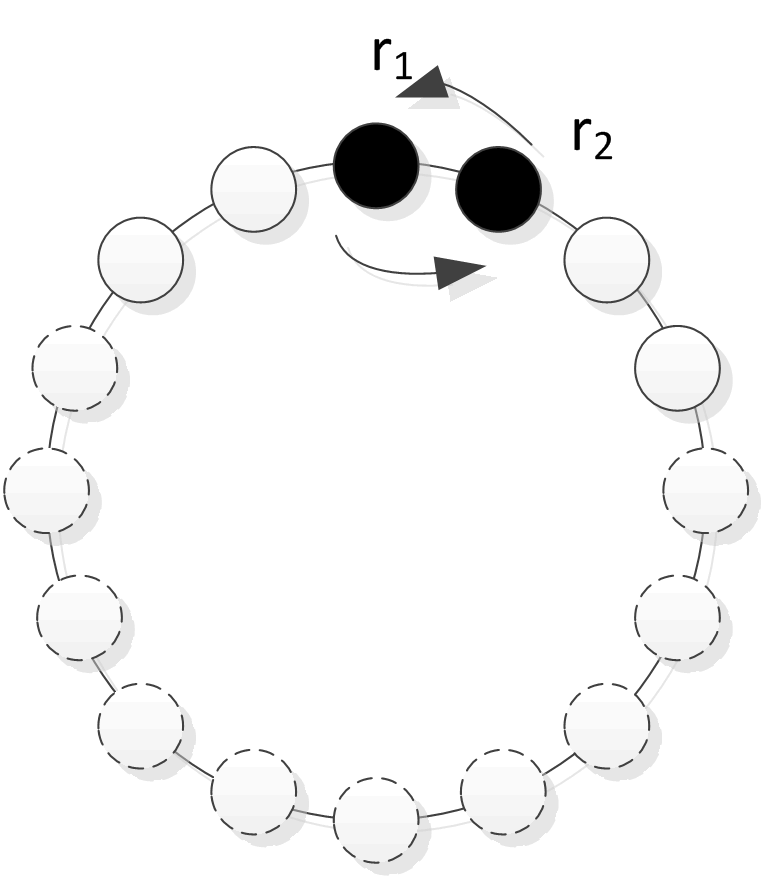
\includegraphics[width=2.5 in]{fig/switch.png}
	\caption{互换}
	\label{fig:switch}
\end{figure}

如图\ref{fig:switch}所示,机器人$r_1$和$r_2$同时相对移动,导致下一个状态时,机器人的位置发生的互换。非互换性是指这种机器人互换空间位置的情况在机器人移动过程中,永远不会发生。

\subsection{非终止性}
非终止性包含两层意思:第一层意思是,空间中每个机器人对空间中的每个位置结点都进行访问;第二层意思是,每个机器人对每个空间位置结点进行重复的访问,而且是永不停止的重复。

\section{本章小结}
本章节介绍了离散空间模型中,自主移动机器人的移动,分别对机器人的三个移动阶段:观察、计算和移动,进行了详细的介绍。对机器人的三种调度策略:半同步调度策略、完全同步调度策略和完全异步调度策略进行了描述。对环形空间和环形空间快照、最小移动算法分别进行了介绍和举例。最后,介绍了永恒探索的三条性质。
